\subsection{Структура библиотеки}

На рисунке \ref{fig:uml} показана структура классов разработанной библиотеки. Классы \texttt{AlgorithmPowerCenter}, \texttt{AlgorithmSphereIntersection} и \texttt{Algorithm\-AGA} являются Objective-C-обертками над одноименными С-классами, содержащими реализации алгоритмов.

\begin{figure}[h!]
    \centering
    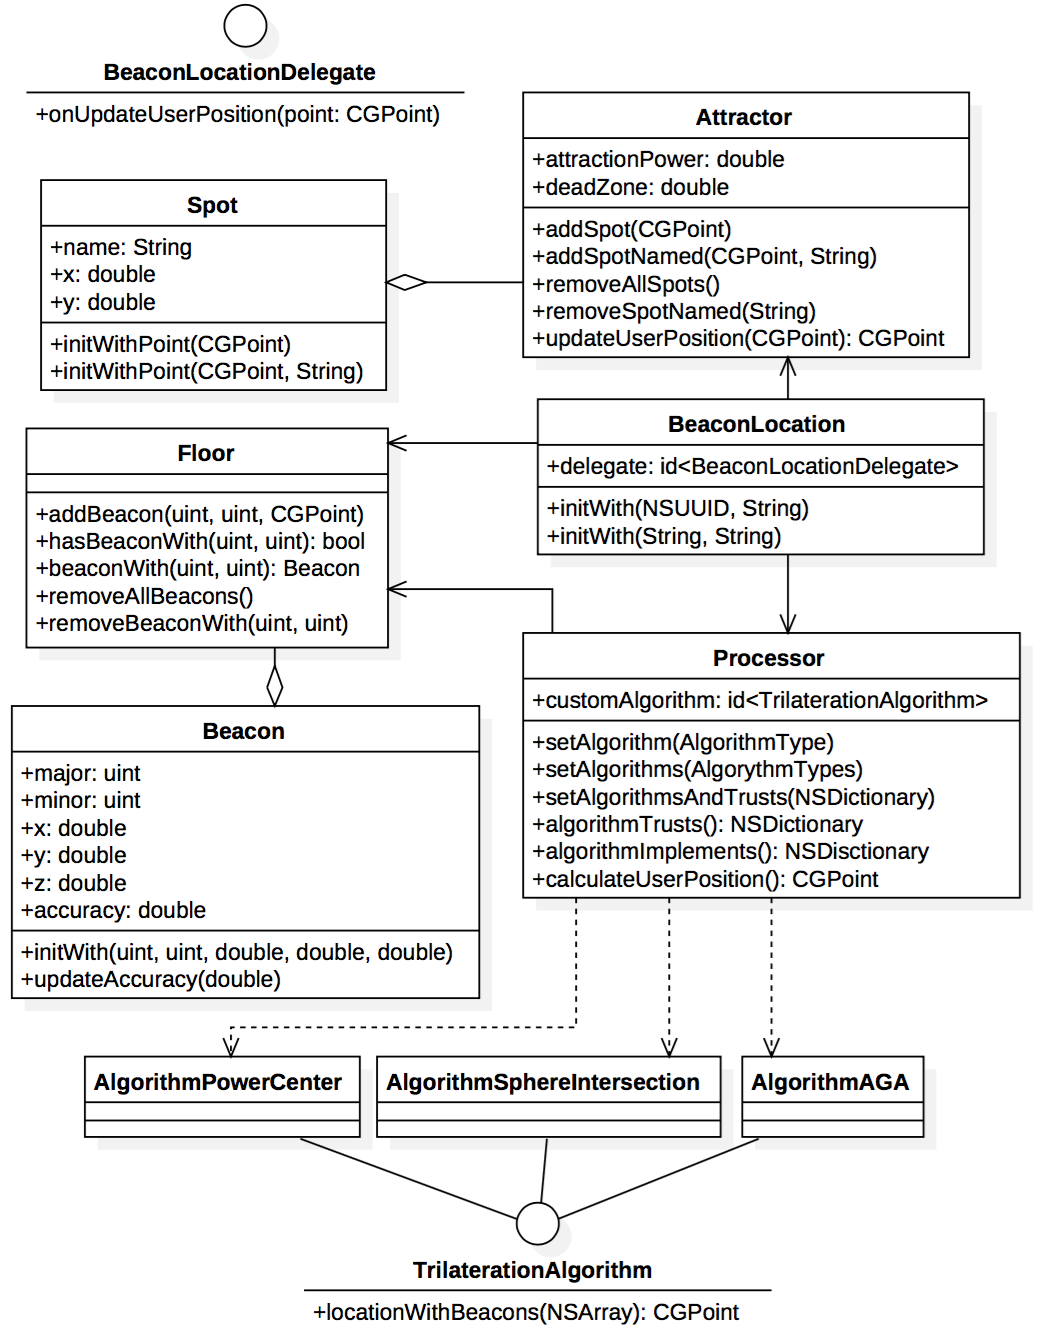
\includegraphics[scale=0.7]{img/uml2}
    \caption{Диаграмма классов разработанной библиотеки}
    \label{fig:uml}
\end{figure}

Пользователь может начать работу с библиотекой двумя способами:
\begin{enumerate}
    \item
    Вручную скопировав все файлы с исходными кодами библиотеки в собственный проект. Следует отметить, что программисты, использующие как Objective-C, так и Swift в своих проектах, могут подключить разрабатываемую библиотеку.
    \item
    Подключив библиотеку через менеджер управления зависимостей Cocoa\-Pods.
\end{enumerate}

После этого он может приступить к первоначальной настройке в рамках приложения: инстанцировать объект библиотеки, добавить необходимую информацию о маячках и подписавшись на обновление пользовательской локации.

Данная процедура проиллюстрирована листингом в приложении 4.